\renewcommand{\theequation}{\theenumi}
\begin{enumerate}[label=\thesubsection.\arabic*.,ref=\thesubsection.\theenumi]
\numberwithin{equation}{enumi}
\item \begin{align}
\vec{P_1} &= \myvec{6\\-6}\\
\vec{P_2} &= \myvec{3\\-7}\\
\vec{P_3} &= \myvec{3\\3}
\end{align}

\item The general of a circle equation is $x^2 + y^2 + Dx + Ey + F$, the equation can be represented as follow in the vector form:
\begin{align}
\vec{x}^T 
\myvec{
1 & 0 \\
0 & 1
}
\vec{x} + 
\myvec{
D & E 
}
\vec{x} + F = 0 \label{eq:general_circle}
\end{align}

Substituting the $P_1, P_2, P_3$ in equation \ref{eq:general_circle}
\begin{align}
\myvec{
6 & -6 & 1\\
3 & -7 & 1\\
3 & 3 & 1}\myvec{D\\E\\F} &= \myvec{-72\\-58\\-18}
\end{align}   

To find D, E, F:
\begin{align}
\myvec{6 & -6 & 1 & -72 \\
3 & -7 & 1 & -58 \\
3 & 3 & 1 & -18
}
&\xleftrightarrow[]{R_1 \leftarrow \frac{R_1}{6}}
\myvec{1 & -1 & \frac{1}{6} & -12 \\
3 & -7 & 1 & -58 \\
3 & 3 & 1 & -18
}\\
&\xleftrightarrow[R_3 \leftarrow R_3 - 3R_1]{R_2 \leftarrow R_2 - 3R_1}
\myvec{1 & -1 & \frac{1}{6} & -12 \\
0 & -4 & \frac{1}{2} & -22 \\
0 & 6 & \frac{1}{2} & 18
}\\
&\xleftrightarrow[R_2 \leftarrow R_2 - R_3]{R_1 \leftarrow R_1 - \frac{R_3}{3}}
\myvec{1 & -3 & 0 & -18 \\
0 & -10 & 0 & -40 \\
0 & 6 & \frac{1}{2} & 18
}
\end{align}

\begin{align}
&\xleftrightarrow[R_2 \leftarrow \frac{-R_2}{10}]{R_3 \leftarrow 2R_3}
\myvec{1 & -3 & 0 & -18 \\
0 & 1 & 0 & 4 \\
0 & 12 & 1 & 36
}\\
&\xleftrightarrow[R_1 \leftarrow R_1 + 3R_2]{R_2 \leftarrow R_3 - 12 R_2}
\myvec{1 & 0 & 0 & -6 \\
0 & 1 & 0 & 4 \\
0 & 0 & 1 & -12
}\\
\implies D &= -6\\
\implies E &= 4\\
\implies F &= -12
\end{align}

\begin{align}
\vec{O} &= \frac{-1}{2A}\begin{pmatrix}
D \\ E 
\end{pmatrix}\label{eq:center_for_circle_ex}
\end{align}

Substituting values of D and E in equation \ref{eq:center_for_circle_ex}
\begin{align}
\therefore \vec{O} &= \myvec{3\\-2}
\end{align}

\item \begin{figure}[!ht]
\centering
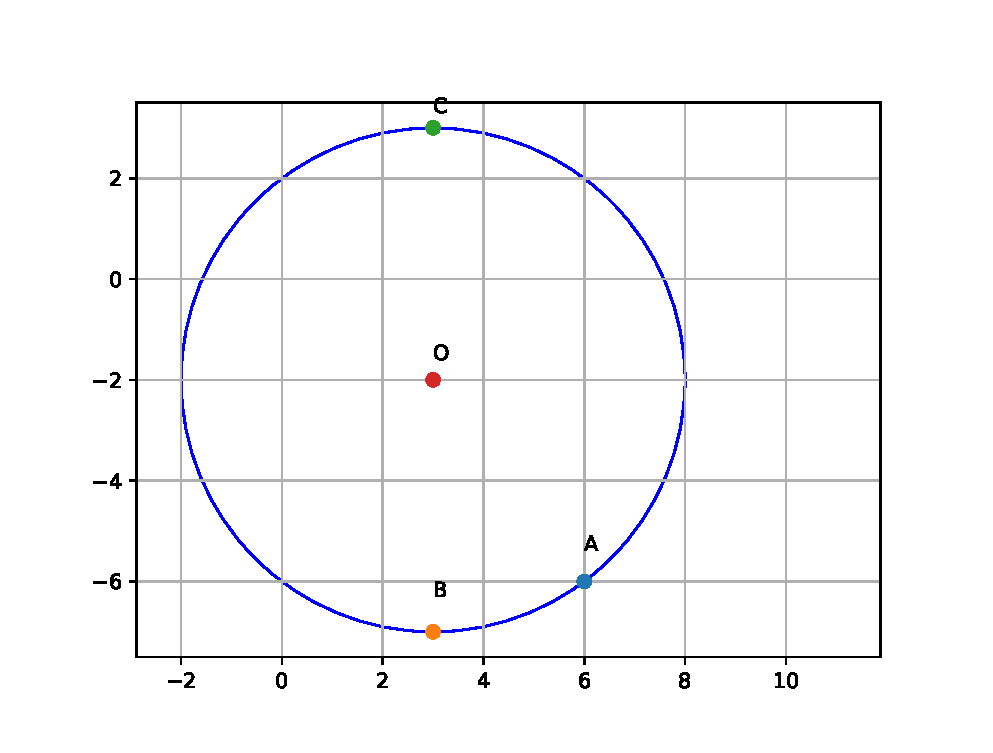
\includegraphics[width=\columnwidth]{./figs/circle_ex/circumcircle.eps}
\caption{Circumcircle generated using python}
\label{fig:Circumcircle2_circle_ex}
\end{figure} 

The following Python code generates Fig. \ref{fig:Circumcircle2_circle_ex}

\begin{lstlisting}
codes/circle_ex/circumcircle.py
\end{lstlisting}
\end{enumerate}



